% !TeX encoding = UTF-8
% !TeX program = lualatex
% !TeX spellcheck = en_US
% !TeX root = thesis.tex

\chapter{Geometric models}
\label{chap:geometric_models}

The following pages contain the various geometry models used for both the validation study as well as BRAC University. The description of the validation study is to be found in \fref{chap:validation_&_verification_study}, the study for BRAC University in \fref{chap:case_study_BRAC_U}.




\clearpage




\begin{figure}[!h]
	\section{Validation study}
	\centering
	\includegraphics[height=1.5\linewidth, trim = 0cm 5cm 10cm 2cm ,clip]{images/geometry/validation/Validation_scaled_down_4P}
	\captionsetup{format=plain}	
	\caption[Geometry used for the validation study; top-view and front-view]{Geometry used for the validation study. Top-view and front-view of validation domain. The dimensions are given in \si{\metre}.}
	\label{fig:validationscaleddown4p}
\end{figure}



\begin{figure}[!h]
	\centering
	\subfloat[][]{
		\includegraphics[width=1\linewidth, trim = 4cm 10cm 2.5cm 11cm , clip, angle= -0.5]{images/geometry/validation/Validation_scaled_down_domain}}\\
	\subfloat[][]{
		\includegraphics[width=.6\linewidth, trim = 5cm 8.5cm 4cm 12cm , clip]{images/geometry/validation/Validation_scaled_down_building}}
	\captionsetup{format=plain}	
	\caption[Geometry used for the validation study; perspective views]{Perspective views of validation geometry  \citep{Jiang2003}. \textbf{(a)} Perspective view of the simulation domain and the vertical samples used; \textbf{(b)} The dimensions of the building within the domain are given in \si{\metre}.}
	\label{fig:validationscaleddownbuilding}
\end{figure}




\clearpage
\chapter{Validation study}
\section{Turbulence models}
\label{sec:appendix_turbulence_study}


The full samples of the validation study of different turbulence models are shown on the following pages.
For the full description of the study, the reader is referred to \fref{sec:validation_turbulence_modelling}. The general boundary conditions of the model can be found in \fref{tab:boundary_conditions_validation_study}.





%\cleardoublepage
\cleartoleftpage
\enlargethispage{3cm}
\includepdf[pages=4,clip,trim=0cm 1cm 21cm -1cm,,noautoscale,fitpaper=false, pagecommand*={\subsection{\kEps\  model}\label{app:plots:kEps}\thispagestyle{plain}\null\vspace*{20cm}\captionof{figure}{\kEps\  turbulence model}}]{images/plots/validation/validation.pdf}
\includepdf[pages=4,clip,trim=21cm 1cm 0cm -1cm,,noautoscale,fitpaper=false, pagecommand={} ]{images/plots/validation/validation.pdf}
%\captionof{figure}{Graphical Illustration of Dataset with an Arbitrary Caption to Highlight the Problem}
\clearpage



\clearpage

\begin{figure}[htbp]
	\section{Mesh refinement}
	\index{validation!LIC}
	\center \hfill 
	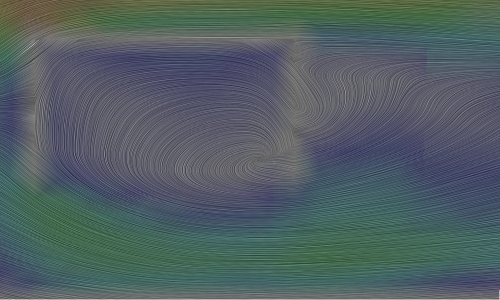
\includegraphics[height=4cm, trim= -1cm 0cm 0cm 0cm, clip]{images/validation/refinement/mod/case_ultra_coarse}
	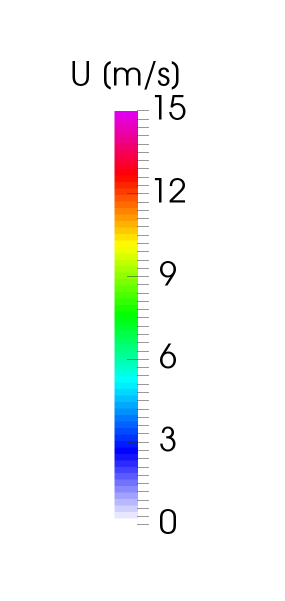
\includegraphics[width=0.15\linewidth]{images/validation/refinement/mod/scale_U}	
	\hfill 
	\noindent\parbox[b][4cm][c]{2cm}{
		\subfloat[\mbox{very coarse}]{}
	} \vspace*{0.5cm}   \\  \hfill 
	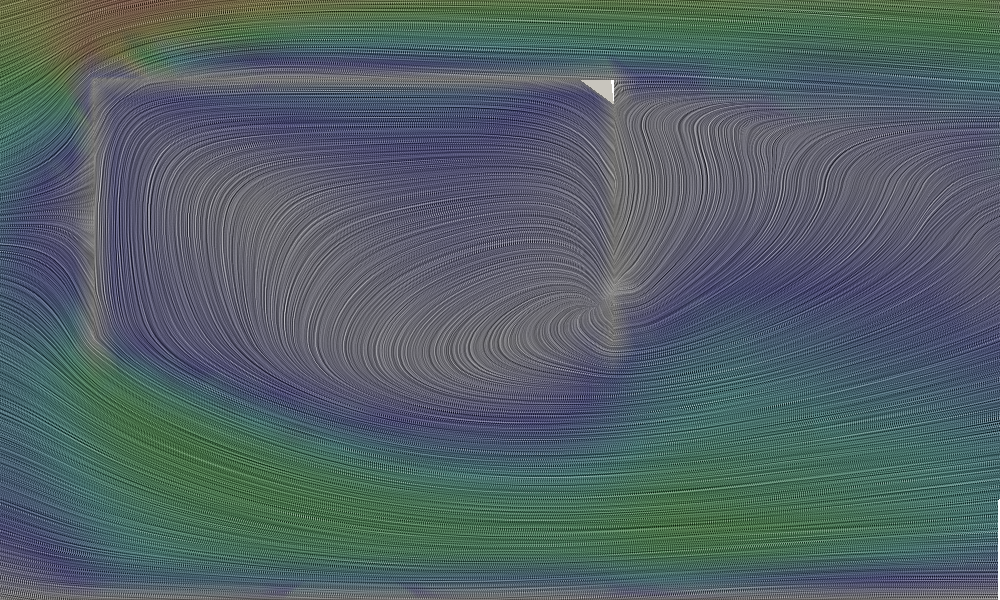
\includegraphics[height=4cm]{images/validation/refinement/mod/case_coarse}
	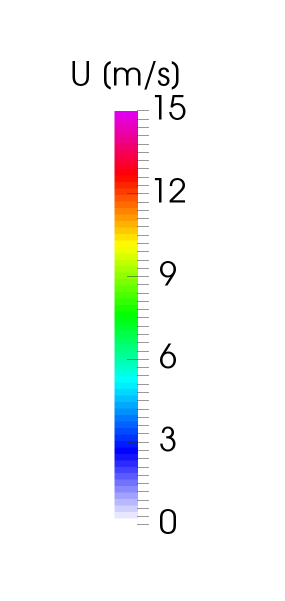
\includegraphics[width=0.15\linewidth]{images/validation/refinement/mod/scale_U}
	\hfill 
	\noindent\parbox[b][4cm][c]{2cm}{
		\subfloat[coarse]{}
	}\vspace*{0.5cm}   \\ \hfill 
	\begin{annotatedFigure}
		{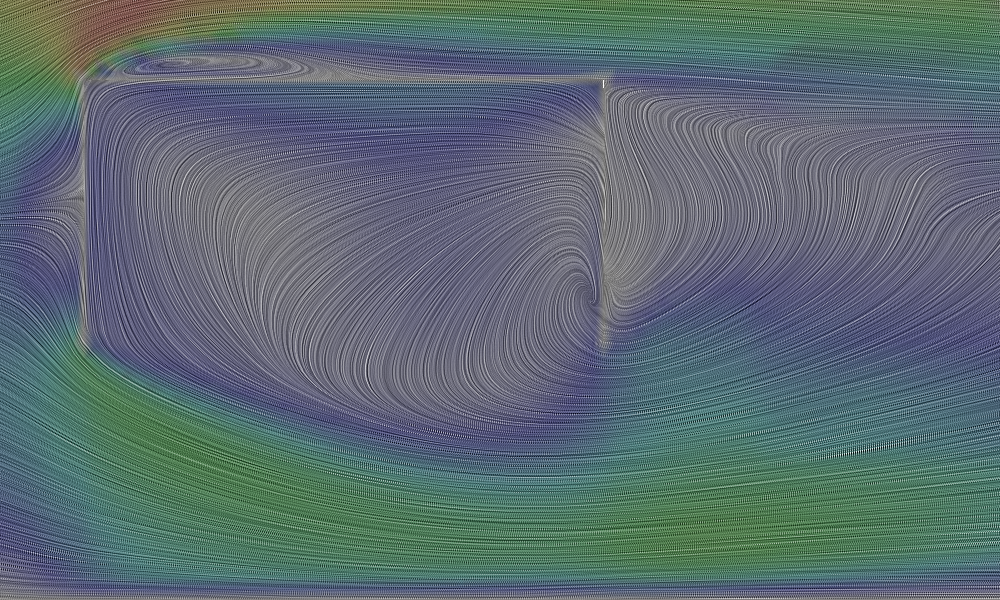
\includegraphics[height=4cm]{images/validation/refinement/mod/case_ref}}
		\annotatedFigureBox{0.091,0.7783}{0.343,0.9683}{A}{0.091,0.80}%bl
	\end{annotatedFigure}
	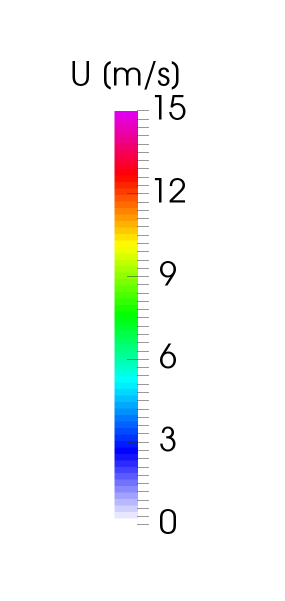
\includegraphics[width=0.15\linewidth]{images/validation/refinement/mod/scale_U}	
	\hfill
	\noindent\parbox[b][4cm][c]{2cm}{
		\subfloat[\mbox{normal}]{}
	} \vspace*{0.5cm}      \\  \hfill 
	\begin{annotatedFigure}
		{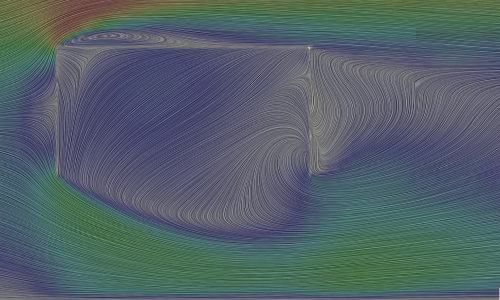
\includegraphics[height=4cm, trim= 2cm 0cm 0cm 0cm, clip]{images/validation/refinement/mod/case_fine}}
		\annotatedFigureBox{0.185,0.4634}{0.48,0.7416}{B}{0.185,0.4634}%bl
	\end{annotatedFigure}
	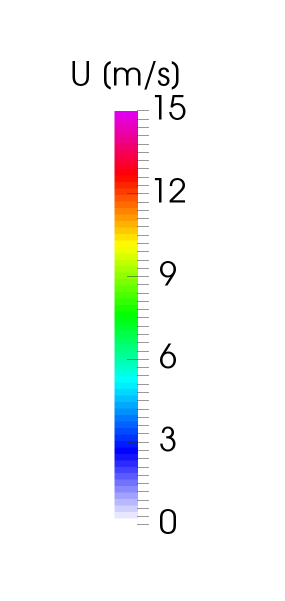
\includegraphics[width=0.15\linewidth]{images/validation/refinement/mod/scale_U}
	\hfill	
	\noindent\parbox[b][4cm][c]{2cm}{
		\subfloat[fine]{}
	}
	\begin{tikzpicture}[scale=1.5]
	\begin{scope}[overlay]
	\draw [->] (-9,1) -- (-8.7,1) node [below] {$y$};
	\draw [->] (-9,1) -- (-9,1.3) node [left] {$z$};
	\end{scope}			
	\end{tikzpicture}
	\captionsetup{format=plain}
	\caption[Flow pattern visualized by the LIC filter for all 4 stages of refinement]{Flow pattern visualized by the LIC filter for all 4 stages of refinement. Depicted is a vertical section through building of validation study. The flow direction is set in the positive y-direction. Both the normal and the find grid are able to resolve the standing vortex just above the geometry (\textbf{A}). The flow pattern in the geometry differs significantly for the fine mesh (\textbf{B}).}
	\label{fig:validation:grid_sens_LIC}
\end{figure}








\clearpage
\chapter{Tables}
\label{app:tables}
\renewcommand{\arraystretch}{1.2} %More linespacing for tables

\clearpage

	\begin{table}[h]
	\caption{Table with footnotes on the same page.}
	\begin{center}
		\begin{threeparttable}
			\begin{tabular}{c c c c}
				\toprule
				\textbf{1st Column} & \textbf{2nd Colimn} & \textbf{3rd Colimn} & \textbf{4th Colimn} \\ \midrule
				QWERTY\tnote{1}   &                     &                     &  \\
				ASDFGH\tnote{2}   &                     &                     &  \\ \bottomrule
			\end{tabular}
			\begin{tablenotes}
				\item[1] qwerty; \item[2] asdfgh
			\end{tablenotes}
		\end{threeparttable}
	\end{center}
	\label{table:simDisimCoefNewDef}
\end{table}

\clearpage


\input{tables/aerodynamic_roughness_length.tex}
